\documentclass[10pt,a4paper]{article}
\usepackage[utf8]{inputenc}
\usepackage[portuguese]{babel}
\usepackage{amsmath}
\usepackage{amsfonts}
\usepackage{amssymb}
\usepackage{graphicx}
\usepackage{url}
\usepackage{makeidx} 
\usepackage{indentfirst}

\title{\Huge\textbf{Redes Neuronais para Reconhecimento de Linguagem Gestual}\linebreak\linebreak\linebreak
\Large\textbf{Relatório Intercalar}\linebreak\linebreak
\Large{Inteligência Artificial}\linebreak
\Large{3º ano do Mestrado Integrado em Engenharia Informática e Computação} \linebreak \linebreak}
\author{\textbf{Elementos do Grupo:}\\ Diogo Joaquim Pinto – 201108016 - ei11120@fe.up.pt \\ Luís Brochado Pinto dos Reis – 201003074 - ei11009@fe.up.pt \\ Wilson da Silva Oliveira - 201109281 - ei11085@fe.up.pt}
\date{28 de Maio de 2014}

\begin{document}

\begin{figure}
\centering

\includegraphics[width=0.7\linewidth]{./LogoFeup}
\end{figure}

\maketitle

\tableofcontents

\newpage

\section{Objetivo}

Este projeto visa a criação de um programa que seja capaz de aprender e reconhecer a linguagem gestual Australiana  (Auslan), utilizando dados com origem numa camera e num par de luvas com capacidade de efetuar medições de alta precisão, recorrendo às capacidades de aprendizagem não-simbólica das redes neuronais.

\section{Descrição}

\subsection{Dataset}

\subsubsection{Parâmetros}

Através da utilização da camera e das luvas de medição foram obtidos onze parâmetros diferentes para cada mão, perfazendo um total de vinte e dois parâmetros que serão processados pela aplicação.

\begin{itemize}
\item Posição X expressa em metros, em relação a uma origem definida ligeiramente abaixo do queixo;
\item Posição Y expressa em metros, em relação a uma origem definida ligeiramente abaixo do queixo;
\item Posição Z expressa em metros, em relação a uma origem definida ligeiramente abaixo do queixo;
\item Rotação no eixo do X, medida num valor entre -0.5 e 0.5, sendo 0 a posição da palma da mão plana horizontalmente. Se o valor for positivo significa que a palma da mão está virada para cima na perspetiva do signatário. Para obter a medida em graus, multiplicar por 180;
\item Rotação no eixo dos Y, medida num valor entre -1.0 e 1.0, sendo 0 a posição da palma para a frente na perspetiva do signatário;
\item Curvatura do dedo polegar medida entre 0 e 1, sendo que 0 significa o dedo esticado e 1 o dedo totalmente dobrado;
\item Curvatura do dedo indicador medida entre 0 e 1, sendo que 0 significa o dedo esticado e 1 o dedo totalmente dobrado;
\item Curvatura do dedo médio medida entre 0 e 1, sendo que 0 significa o dedo esticado e 1 o dedo totalmente dobrado;
\item Curvatura do dedo anelar medida entre 0 e 1, sendo que 0 significa o dedo esticado e 1 o dedo totalmente dobrado;
\item Curvatura do dedo mindinho medida entre 0 e 1, sendo que 0 significa o dedo esticado e 1 o dedo totalmente dobrado.
\end{itemize}
\textbf{É assinalado na fonte da base de dados que as medidas de dobra dos dedos não são totalmente exatas}.

\subsubsection{Normalização dos dados}

O dataset necessitou de algumas normalizações, de modo a que todos os valores se encontrassem \textbf{entre 0 e 1}, nomeadamente em:
\begin{itemize}
\item X, Y, Z aplicou-se o módulo
\item Rotação no eixo do X incrementou-se 0.5 aos valores
\item Rotação no eixo do Y incrementou-se 1 e tirou-se a metade
\end{itemize}

\subsubsection{Processamento do Dataset}

A base de dados contém um total de \textbf{95} palavras com \textbf{27} amostras para cada uma totalizando assim \textbf{2565} amostras.
Cada amostra contém em média \textbf{60} medições únicas (correspondentes aos frames captados pelos dispositivos de medição) dos 22 parâmetros especificados anteriormente.
Dado o elevado número de dados optamos por processar a média destes valores, numa tentativa de reduzir a carga sobre a rede neuronal, mas com o cuidado de garantir valores únicos para cada palavra diferente. Para tentar eliminar os frames menos essenciais para o gesto (que seriam os frames iniciais e finais), optamos por eliminar estes do cálculo da média final.

Para possibilitar o teste da aplicação nos nossos computadores "modestos" utilizamos uma versão reduzida da base de dados com apenas 8 palavras ao invés das \textbf{95} disponibilizadas. Não consideramos tal prejudicial visto que isto é uma \textit{proof of concept}

\subsection{Arquitectura da Rede Neuronal}

Existem 3 tipos de de rede neuronal, redes totalmente conectadas, redes de camada única e redes de múltiplas camada.
Optamos pela implementação de \textbf{redes de camada múltipla}, visto que os dados não são linearmente separáveis; e permitiria a implementação de sub-redes, caso o dataset permitisse a associação entre parâmetros, o que levaria a um incremento na eficiência da rede neuronal; e é a qual, dado ser mais comummente utilizada, tem mais heurísticas e recursos desenvolvidos.

As camadas de entrada e de saída possuíam logo à partida valores fixos:
\begin{itemize}
\item a camada de entrada possui 22 nós, um por cada input
\item a camada de saída possui 8 nós (no caso da base de dados reduzida), um por cada palavra
\end{itemize}

Após investigação sobre o tema com especialistas, não foi possível concluir qualquer associação entre os parâmetros relevantes.

Dado isto, foram testadas inúmeras arquiteturas, incluindo redes totalmente conexas com mais e menos nós na camada intermédia, bem como outras topologias: numa delas, como tentativa de agregação de informação, a camada intermédia recebia os dados dos nós da camada de entrada como se segue:
\begin{itemize}
\item posição (x, y, z) das duas mãos
\item dobra dos dedos polegar, indicador e médio da mão esquerda
\item dobra dos dedos polegar, indicador e médio da mão direita
\item dobra dos dedos anelar e mindinho da mão esquerda
\item dobra dos dedos anelar e mindinho da mão direita
\item rotações no espaço da mão esquerda
\item rotações no espaço da mão direita
\item dois nós com todos os parâmetros
\end{itemize}

\begin{figure}[here]
\centering
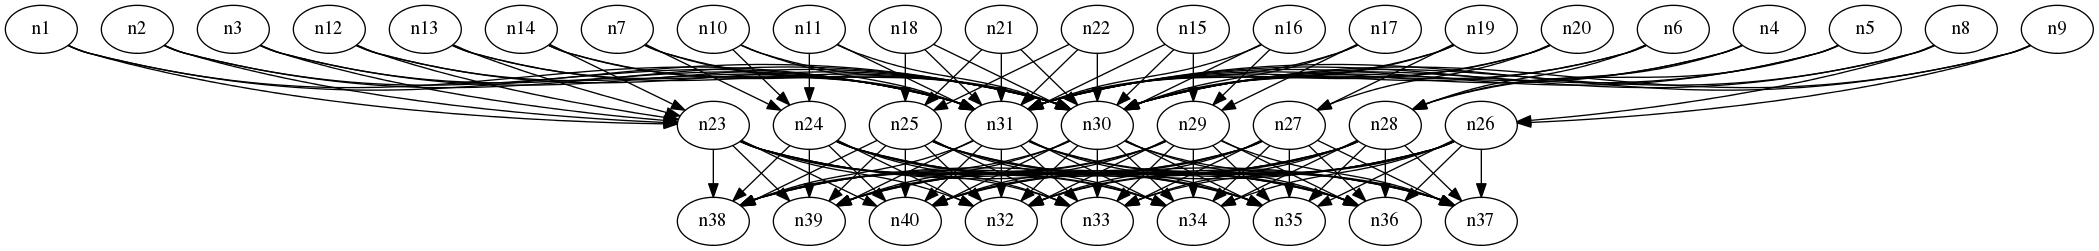
\includegraphics[scale=0.15]{net2.png}
\caption{Primeira rede neuronal final}
\end{figure}

Após vários testes, acabamos com esta arquitetura como uma das finais: a outra é totalmente conexa e continha uma \textbf{camada intermédia única de 5 nós}.
\\
\begin{figure}[here]
\centering
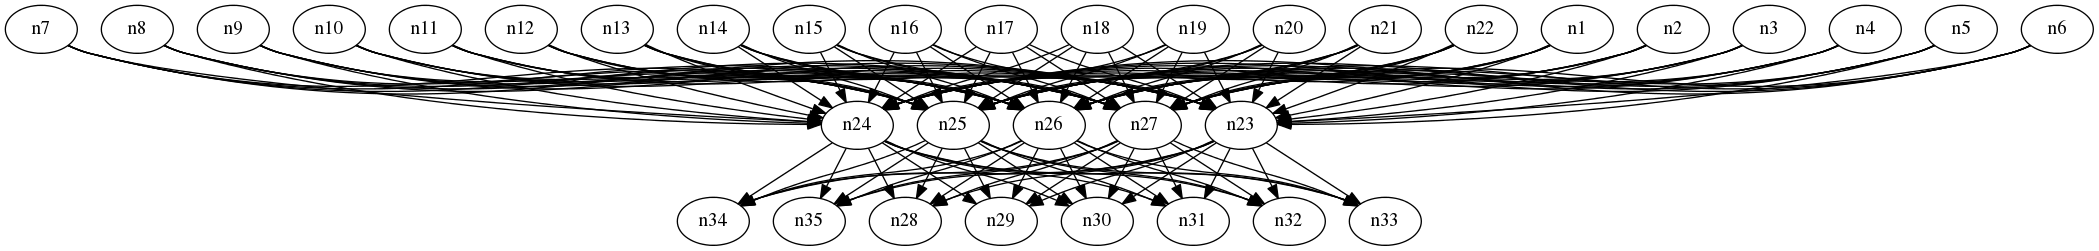
\includegraphics[scale=0.15]{net1.png}
\caption{Segunda rede neuronal final}
\end{figure}

\subsubsection{Backpropagation}

\begin{figure}[here]
\centering
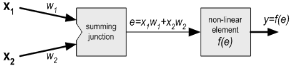
\includegraphics{neuron.png}
\caption{Exemplo de neurónio individual}
\end{figure}

O algoritmo de backpropagation é um método do tipo feedforward.
Dado isto, inicialmente propaga-se os parâmetros recebidos na camada de entrada pelas ligações. Nas camadas intermédias e na camada de saída, om \textit{impulsos} são somados e em seguida aplica-se uma função de transferência à medida que transmite os dados às camadas seguintes.

\begin{figure}[here]
\centering
\[s_{i} = \tfrac{1}{1 + e^{\sum_{k=1}^{m}v_{k} * p_{k}}}\]
\caption{Transferência (sigmóide) com base na soma ponderada (pelos pesos) dos valores recebidos nas arestas}
\end{figure}

Chegando os \textit{impulsos} à camada de saída, informação é retro-propagada para trás até à camada de entrada: após o cálculo dos erros na camada de saída, os erros são propagados para as camadas intermédias e à medida que o erro vai sendo propagado para trás, o peso das ligações entre camadas é alterado de modo a diminuir o erro. Este passo também é conhecido como "Treino" da rede.

Atualizar o peso das ligações (é equivalente a minimizar o erro) é o modo de se reduzir para zero, ou aproximadamente zero, o erro na camada de saída, tornando a rede neuronal fidedigna.

\begin{figure}[here]
\centering
\[\varpi _{it} = \varpi _{it - 1} + \eta * \delta * \frac{\partial f(e)}{\partial e}*y\]
\caption{Cálculo do novo peso da aresta}
\end{figure}

Este processo é feito através da função de custo quadrático e da sua derivada, sendo que a primeira é a função a minimizar no algoritmo de retropropagação (apresentando \textbf{\textit{x}} exemplos a um rede com \textbf{\textit{y}} saídas).

% TODO 

\subsection{Condição de paragem da aprendizagem}

A aprendizagem é feita sobre a base de dados em ciclo, parando apenas quando uma iteração sobre todas as amostras de aprendizagem produz resultados corretos nos nós de saída. Definimos como resultados válidos na aprendizagem quando a diferença entre o valor mais alto na camada de saída difere de pelo menos \textbf{0.3} unidades do segundo mais alto.
Já no teste, a diferença entre estes valores não tem qualquer restrição (de modo a potenciar a \textbf{generalização}).

\section{Estruturação da aplicação}
\begin{figure}[here]
\centering
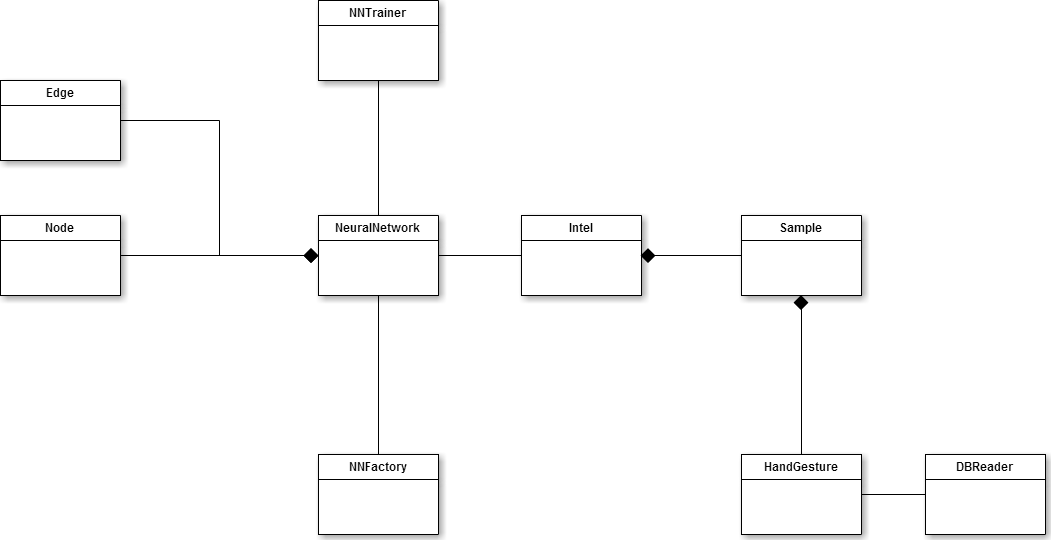
\includegraphics[scale=0.33]{iart_nn.png}
\caption{Diagrama de classes}
\end{figure}

\section{Medições}

\subsection{Variação da velocidade de aprendizagem}

Após vários testes, concluimos que o valor onde a aprendizagem era feita com menos flutuações, maximizando a rapidez da aprendizagem, era com o valor de \textbf{0.3}. Valores superiores implicavam uma aprendizagem deficiente.

\subsection{Resultados com a variação da quantidade de exemplos fornecidos}

Foi necessário verificar a validade de cada caso na seguinte equação:

\begin{figure}[here]
\centering
\[L<S*E\]
L $\rightarrow$ nº de ligações \\ S $\rightarrow$ nº de saídas \\ E $\rightarrow$ nº de exemplos de aprendizagem
\end{figure}

Sendo que 
\begin{figure}[here]
\centering
\[S*E = N\]
N $\rightarrow$ nº de equações
\end{figure}


\begin{tabular}{|c|c|c|}
\hline 
da BD para aprendizagem & Resultado & Verifica \\ 
\hline 
11 & 216 $<$ 192 & Não \\ 
22 & 216 $<$ 384 & Sim \\ 
33 & 216 $<$ 576 & Sim \\ 
44 & 216 $<$ 768 & Sim \\ 
56 & 216 $<$ 960 & Sim \\ 
67 & 216 $<$ 1152 & Sim \\ 
78 & 216 $<$ 1344 & Sim \\ 
89 & 216 $<$ 1536 & Sim \\ 
\hline
\end{tabular} 

É possível concluir que, para 11\% da base de dados para aprendizagem, não existem exemplos suficientes para a rede neuronal \textbf{generalizar}, pelo que tende apenas a adaptar-se às equações lineares que modelam as soluções.


\section{Conclusões}

Após a realização deste projeto/investigação foi possível comprovar a influência da variação de parâmetros como a \textbf{velocidade de aprendizagem} e o \textbf{número de exemplos de aprendizagem}. Identificamos ainda a importância e o poder da capacidade de generalização e de tratamento de informação não simbólica das redes neuronais. Porém, esta mesma natureza leva a que não nos seja possível obter explicações para as conclusões que ela retira.

\section{Possíveis Melhorias}
\subsection{Modificação do cálculo do erro}
A inclusão no cálculo do erro de uma iteração de aprendizagem pela rede neuronal da derivada da função sigmóide levaria a uma aprendizagem acelerada nos valores intermédios e lenta perto dos valores limite (0 e 1), sendo que um exemplo já aprendido, no backpropagation não iria alterar em demasia os valores dos pesos, contribuindo para a estabilidade da rede. 

\subsection{Cálculos através da GPU}
Uma hipótese de aumentar a rapidez de treino da base de dados seria implementar a execução dos cálculos através da GPU do computador.

\subsection{Variância como parâmetro}
Uma vez que os dados de input são a média das medições dos parâmetros das amostras, a adição do input das variâncias dos respectivos cálculos poderia ser uma mais valia na distinção entre amostras de movimentos dinâmicos e de estáticos. Seria preciso ter em conta, porém, que isto implicaria um aumento no número de arestas da rede, logo uma fase de aprendizagem mais prolongada.

\section{Recursos}

O software utilizado foi o IDE IntelliJ IDEA 13.1.1, para programação em Java.


 \begin{thebibliography}{1}

  \bibitem{diapositivos} Eugénio Oliveira {\em Diapositivos de IART: {\url{http://paginas.fe.up.pt/~eol/IA/1314/APONTAMENTOS/7_RN.pdf}}}  2013-2014.
  
  \bibitem{wiki} Wikipedia, Redes Neuronais Modulares {\em\url{http://en.wikipedia.org/wiki/Modular_neural_network}}.

  \bibitem{livroen} Peter Norvig, Stuart Russell {\em Artificial Intelligence A Modern Approach } 2009: Prentice Hall.
  \end{thebibliography}
  \printindex
\end{document}